\chapter{Numerical Simulation of Heat Transfer} % Main chapter title

\label{Chapter4}

\section{OpenFOAM: chtMultiphaseInterFOAM. Conjugate Heat Transfer}
The last objective of this thesis is to extend the multiphase solver of the previous section so it can account for multiregion purposes. To do so, a new solver derived from the concept of an existing multiregion solver is implemented. The existing solver, \textit{chtMultiRegionFoam} is developed on the basis that the fluid it solves undergoes the compressible Navier-Stokes equations with buoyancy forces and the energy equation per unit mass with gravity terms as follows:
\subsubsection*{Continuity Equation}
\begin{equation}
\frac{\partial \rho}{\partial t}+\nabla \cdot(\rho \boldsymbol{u})=0
\end{equation}
\subsubsection*{Momentum Equation}
\begin{equation}
	\begin{aligned}
		&\frac{\partial \rho \boldsymbol{u}}{\partial t}+\nabla \cdot(\rho \boldsymbol{u} \otimes \boldsymbol{u})=\\
		&-\nabla p_{\mathrm{rgh}}+\nabla \cdot\left[\mu\left\{\nabla \otimes \boldsymbol{u}+(\nabla \otimes \boldsymbol{u})^{\mathrm{T}}\right\}\right]
		-\nabla\left(\frac{2}{3} \mu \nabla \cdot \boldsymbol{u}\right)-\boldsymbol{g} \cdot \boldsymbol{x} \nabla \rho
	\end{aligned}
\centering
\label{4.1}
\end{equation}
\subsubsection*{Energy Equation}
\begin{equation}
\frac{\partial \rho h}{\partial t}+\nabla \cdot(\rho \boldsymbol{u} h)+\nabla \cdot(\rho \boldsymbol{u} K)=\nabla \cdot\left(\frac{\lambda}{c_{p}} \nabla h\right)+\rho \boldsymbol{u} \cdot \boldsymbol{g}
\label{4.2}
\end{equation}
where \textit{\textbf{u}} is the velocity vector, \textit{h} is the enthalpy, \textit{K = 0.5*\textbf{u $\cdot$ u}} is the kinetic energy per unit mass, \textit{$p_{rgh}=p-\rho\textbf{g}\cdot\textbf{x}$} the modified pressure so that the momentum equation accounts for the buoyancy terms, and the remaining thermophysical properties, $\mu$, $\lambda$, $C_p$ being the kinematic viscosity, the thermal conductivity and the specific heat accordingly. The energy equation does not include radiation, heat generation term and chemical reaction.
\newline
Therefore, the challenge of this part is to couple the multiphase solver (\textit{IcoReactingMultiPhaseInterFoam}) that allows for the solving of a fluid undergoing phase-change with a solid region.  
\subsection{Case description}
\subsection{Hypotheses And Assumptions}
\subsection{Governing Equations of the Fluid Region}

\subsection{Governing Equations of the Solid Region}
\subsubsection{Energy Equation}
\begin{equation}
\nabla \cdot\left(\frac{\lambda}{\rho c_{p}} \nabla h\right)=0
\label{4.3}
\end{equation}

\subsection{Solver description. Control Loop}
\begin{figure}[h!]
	\centering
	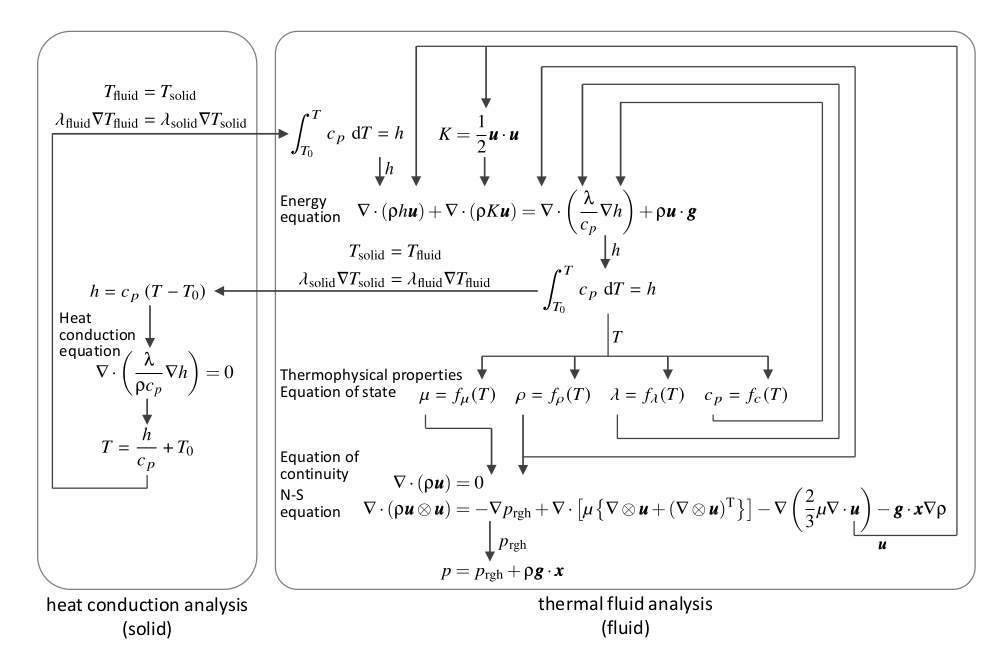
\includegraphics[width=\linewidth]{CHT_flowchart.png}	
	\label{4.1fig}
	\caption{Flowchart of the conjugate heat transfer solver.\cite{sugimoto_kuramae_matsumoto_watanabe_2021}}
\end{figure} 
chtMultiphaseInterFoam is a new solver derived from the existing solver chtMultiRegionFoam. It is implemented to cope with transient fluid flow and solid heat conduction with conjugate heat transfer between regions.
The solution follows a sequential strategy: equations of the fluid are first solved using the temperatures of the solid of the preceding loop to set the boundary conditions for the fluid part.Then, the equation for the solid is solved with the temperatures of the fluid to define lately the boundary conditions of the solid. This process is iteratively executed until convergence is reached.

\subsection{Code implementations}
\subsection{Case Setup}
\subsubsection{Boundary conditions}
At the interface between solid and liquid regions, it is required to set an appropriate boundary condition which couples the energy equations in these areas.
\newline
Considering two cells at each side of the interface such as in the Figure
\newline
where $T_c$ and $T_p$ is the temperature at the cell center and on the patch (2D boundary) accordingly. $q_1$ is the heat flux going out of the $cell_1$ and $q_2$ the heat flux entering the $cell_2$. The energy conservation in this zone constrains the temperature and heat fluxes to be equat at both sides of the interface. 
Then, temperature, in magnitude yields as
\begin{equation}
	T_{p, 1}=T_{p, 2}=T_{p},
	\label{4.4}
\end{equation}
and as well, for the fluxes
\begin{equation}
q_{1}^{\prime \prime}=q_{2}^{\prime \prime}=q^{\prime \prime}
\label{4.5}
\end{equation}
while the magnitude for the heat fluxes is derived from the one-dimensional expression for the Fourier's law and it gives
\begin{equation}
-\left.k_{1} \frac{\partial T}{\partial n}\right|_{\text {side } 1}=-\left.k_{2} \frac{\partial T}{\partial n}\right|_{\text {side } 2}
\label{4.6}
\end{equation}
where $\kappa$ is the termal conductivity and $n$ the direction normal to the patch.
Discretizing linearly the temperature gradient of the previous equation, and with respect of the scheme of the Figure [], the differential equation that yields 
\begin{equation}
k_{1} \Delta_{1}\left(T_{c, 1}-T_{p}\right)=k_{2} \Delta_{2}\left(T_{p}-T_{c, 2}\right)
\label{4.7}
\end{equation}
where the temperatures and fluxes at the center of the patches are described as
\begin{equation}
\begin{gathered}
T_{p}=\frac{k_{1} \Delta_{1} T_{c, 1}+k_{2} \Delta_{2} T_{c, 2}}{k_{1} \Delta_{1}+k_{2} \Delta_{2}} \\
q^{\prime \prime}=k_{1} \Delta_{1}\left(T_{c, 1}-T_{p}\right)=k_{2} \Delta_{2}\left(T_{p}-T_{c, 2}\right) .
\end{gathered}
\label{4.8}
\end{equation}
\subsection{Validation of Results and Conclusions}

